\chapter{Introduction}
\section{Importance of research}
Recent advancement in technology in general has led to the flourishment of many undiscovered industries. Many of them involve with the rapid expansion of the Internet, as an effective channel to reach customers. One of these newcomers is Internet radio broadcasting. For the past 2 years, internet radio has been becoming a new mainstream form of entertainment that attracts a consistent amount 
of listeners and broadcasters. 
\begin{figure}[h]
	\centering
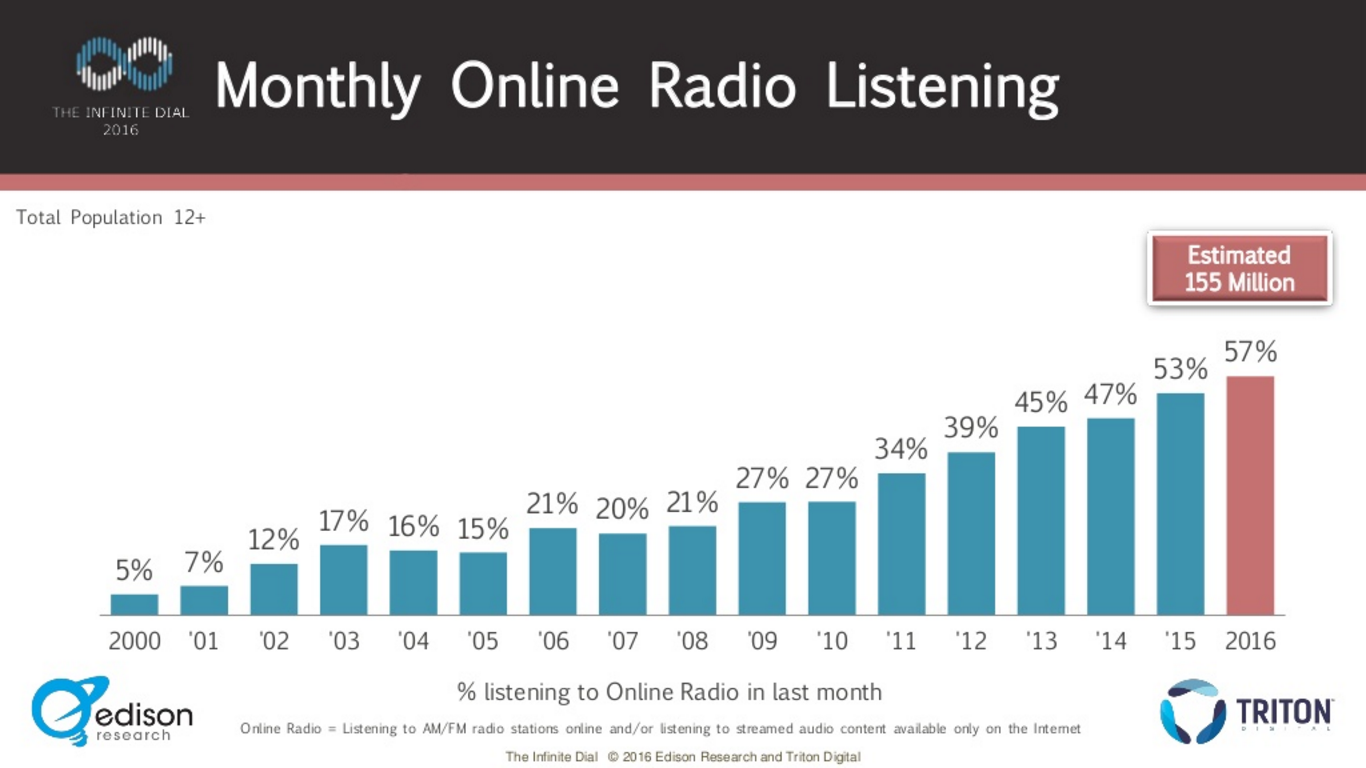
\includegraphics[width=\textwidth]{monthly-online-listening}
 	\caption{Monthly Online Listening. Source\cite{edisonslide}}
 	\label{fig:MonthlyOnlineListening}
\end{figure}
According to Infinite Dial report from Edison Reasearch\cite{edison2016}, the monthly internet radio audience has been constantly increasing for the last 15 years. In 2016, it passed over 50\% the total population that over 12 years old of the U.S, reached 57\%. This fact indicates a undeniable trend in the listening behavior of audience, that there are estimated 155 million people that listen to Internet radio monthly in America. 

In 2016, the reports from the same organization also show interesting data about the number of weekly Internet radio listeners, which rises from 44\% in 2015 to 50\% of respondents age 12 and older in 2016. With 57\% of Americans using online radio monthly in 2016, we can induce to the interesting fact that 88\% of them has made it a weekly habit, this is shown in details in \ref{fig:MonthlyWeekly}. 

From the same report, it tells that Internet radio listening now
averages about 12 hours and 53 minutes per week across
the weekly online radio listeners population in 2015. Listening hours are critical. They
represent opportunities to reach real people with
advertising messages. While according to the XappMedia Internet Radio Ad Load Report in Quater 1 of 2015\cite{xapp2015q1}, it revealed an average of 2 minutes and 18 seconds of ads
per hour. At 12:53 hours of listening per week, that reflects
about 29 minutes of ads. Recent analysis shows the
average Internet radio spot length is 25.88 seconds, which
translates into about 68 ad impressions per week, per
listener. 

It is also reported that 95\% of the audience choose ad-supported listening form. That domination opens a huge number of opportunities for advertisers to reach an engaged audience. In fact, internet radio advertising is the new trend with findings from the Internet Radio Ad Load Report Q4 2015\cite{xapp2015q4}, where the total advertisers indentified through 2015 rose to 406, a 5.4x increase over 2014. This form of advertising plays fewer commercials per hour, which result in higher listener attention levels, increasing the ads, intended effect. Plus, listeners are only one click away from an advertiser's web site. They are online and have browser window open. This makes it very easy to get listeners to visit the advertiser's website. Web radio listeners are also a highly active group of consumers with an above average level of purchase intention.


\begin{figure}[h]
	\centering
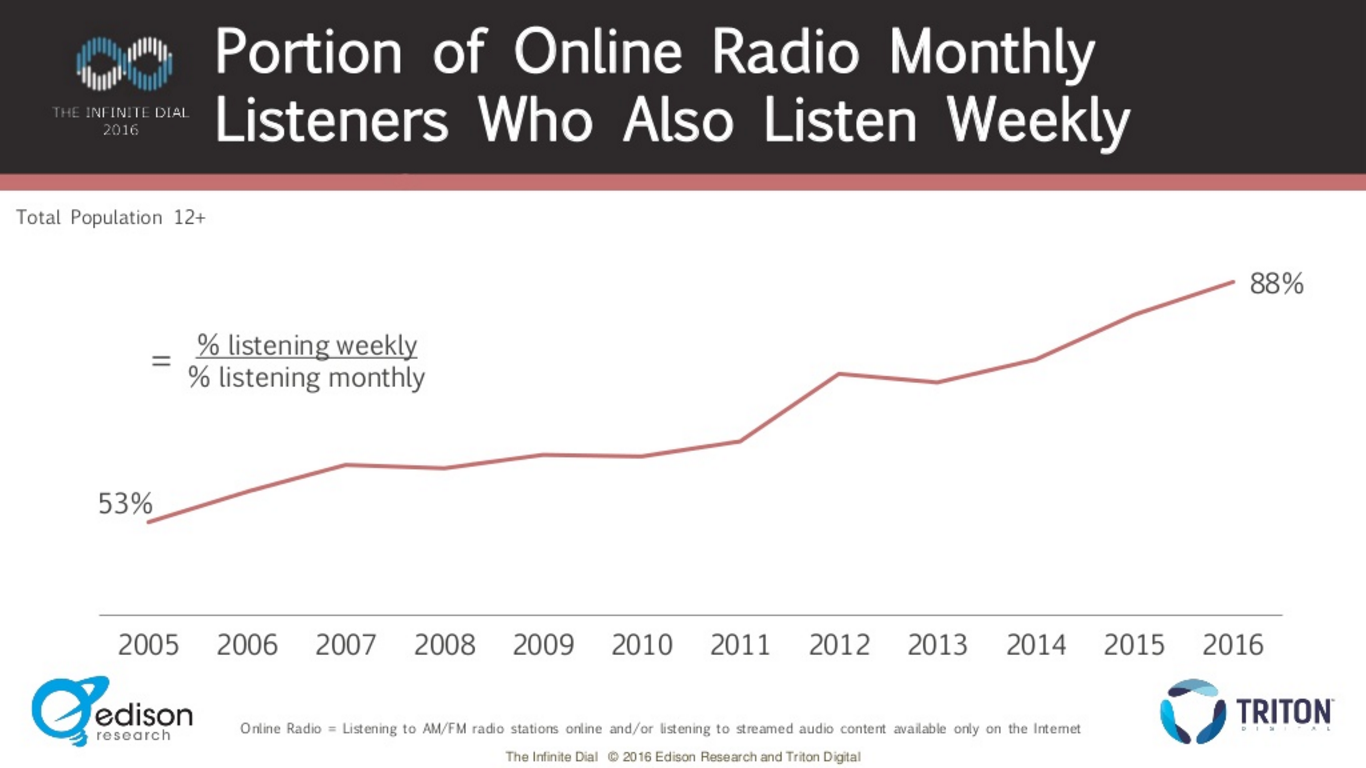
\includegraphics[width=\textwidth]{monthly-weekly}
 	\caption{Monthly online radio listeners who also listen weekly. Source\cite{edisonslide}}
 	\label{fig:MonthlyWeekly}
\end{figure}

For businesses, it is important to reaching out to as many clients as possible. To achieve this, one should capitalize on a type of marketing and focus on enhancing its effectiveness. In the case of internet radio, since it's a relatively new field, research is required to make the most advantage out of this new advertising form. Otherwise, a bad model would not last long due to the fast changing pace tech industry. In such a state, one has to equipped himself with knowledge and tools to be adaptable to different situations.

There are a lot of research one can try to strengthen his advertising system. He can either publish more channels leading to customers, make better content or invest more money into the campaign. For this particular project, we focus on a more scienctific approach, which of course has many trade offs compare to other ones. Open a research and development project, apply the knowledge into a live system are not easy, care must be taken very serisously when such decisions are made. It's important to take everything in the equation, where we can evaluate what's are the trade offs of our research. Otherwise, one might waste time and resources going the wrong path. 

In general, an enhancement in terms of science would question the existing system in a most fundamental way. It is totally possible that one has to replace his whole model for a scienctific solution to come in. And this takes times and a lot of effort. But on the other hand, since it focuses on the root of all causes, not just patching here and there, it would be able to solve classic puzzles that other approaches can not. 

To choose the right path, we should consider the context of our problem, the Internet itself. Rapidly changing in all dimensions, unpredictable and chaotic are the properties of the Internet nowadays. Common businesses are not equipped with necessary tools to deal with this. Therefore, they often find themselves solving problems that keep pops up one after another. Only a scienctific solution can help them in this battle.

\section{Challenges	with traditional radio advertising}

At the time of this research, the popular form of advertising over radio channel is done by inserting an advertising fragment into the streaming buffer. By this way, it produces a stream of media that plays out naturally with autual content separated by advertisements. 

There are many big multimedia streaming companies that use this approach, namely Spotify, Youtube or Apple Music. A good point with this method is its simplicity. Straightforwardly, temporarily pause the stream and play an advertisement until it ends or users explicitly skip. Simple means easy to deploy and get up and running, plug and play with different settings. That would help boost the market research progress or anything favor flash launching. An obvious downside is actively interupting user experience with advertisements. Unless it is a relevant one, user would feel annoyed and skip the advertisement or even leave the session. For established cooperation, they focus on the amount of advertisement views, not necessarily engagement quality, as they already have a tremendous userbase. Hence, this method apparently fits them.

However, for small project, listeners are very important so it's not wise to take risk degrading the user experience. Instead, the advertisement content should be made carefully too, to use as a tool to attract even more users. And this is not something traditional methods are really good at. Plus, there is a classic challenge that any form of advertisement face, it hardly creates any potential audience engagement that could lead to actual advertising success. The traditional system lacks a channel that effectively guide listeners to the advertisers intention rather than mere meaningless advertising audio. And this is what we are trying to solve.

\section {Motivation and Research Aims}

Seeing how promising the industry of Internet radio broadcasting is, it appears urgent that we should propose a systemic solution to help magnify the good points and minimize the bad points of this innovate channel. Internet radio advertising find itself good at providing a cheap way to reach listeners, while also possible to be effective if further consideration in advertising timing and content is made. On the other hand, one of its bad sides is lacking effectiveness in user engagement. In order to optimize this, we need the following points for our system:
\begin{itemize}
\item{On top of our solution, we want to reserve the benefits of traditional Internet radio advertising. That is cheap, simple and easy to implement.}
\item{A way to exhibit more relevant contents that support the advertisement. Traditional way of broadcasting advertisement lacks a space for that kind of extra information. While it appears naturally that pure audio ads are not enough to notice listeners. One might missheard the advertisement and has no way to go back, he has to go online to look for more information. Plus, it's better to have extra information supporting the running advertisement. Listener might want to research further information about pricing, extra options before deciding to buy products from advertisements.}
\end{itemize}

\section {Thesis Outline}
This thesis is comprised of six chapters. A schemantic overview of this thesis is shown in Fig. \ref{fig:ThesisOverview}. Chapters 2-6 are organized as follows.

Chapter 2 presents the background knowledge related to this thesis and the key principles for the proposed approach. It starts with an overview of our solution, then glimpse the needed parts that we need for this project. We also present in details the concepts that we borrow from other fields such as audio data hiding and concurrency programming.

Chapter 3  and 4 show our proposed method based on the background we had describe in Chapter 2. We divide our system into many small part, each with its own section to discuss. In the process, we also bring up many unresolved issues with some classic trade offs, which we rely on experimenting in Chapter 5 to deal with. To provide a intuitively walkthrough of our system, we exhibit many flow charts to resemble the system.

We continue to the testing, experimenting and optimzation in Chapter 5. While Chapter 4 points out several parameters we need to optimize, Chapter 5 propose and execute tests on different settings to determine the best choice. We then provide test results presented in meaningful figures, which would help us make sense of the data and choose our optimal solution. 

Finally, Chapter 6 summarizes this study, gives some concluding remarks, highlights our contributions to the advertising industry, and opens a number of directions for further upgrade to the system.

\begin{figure}
  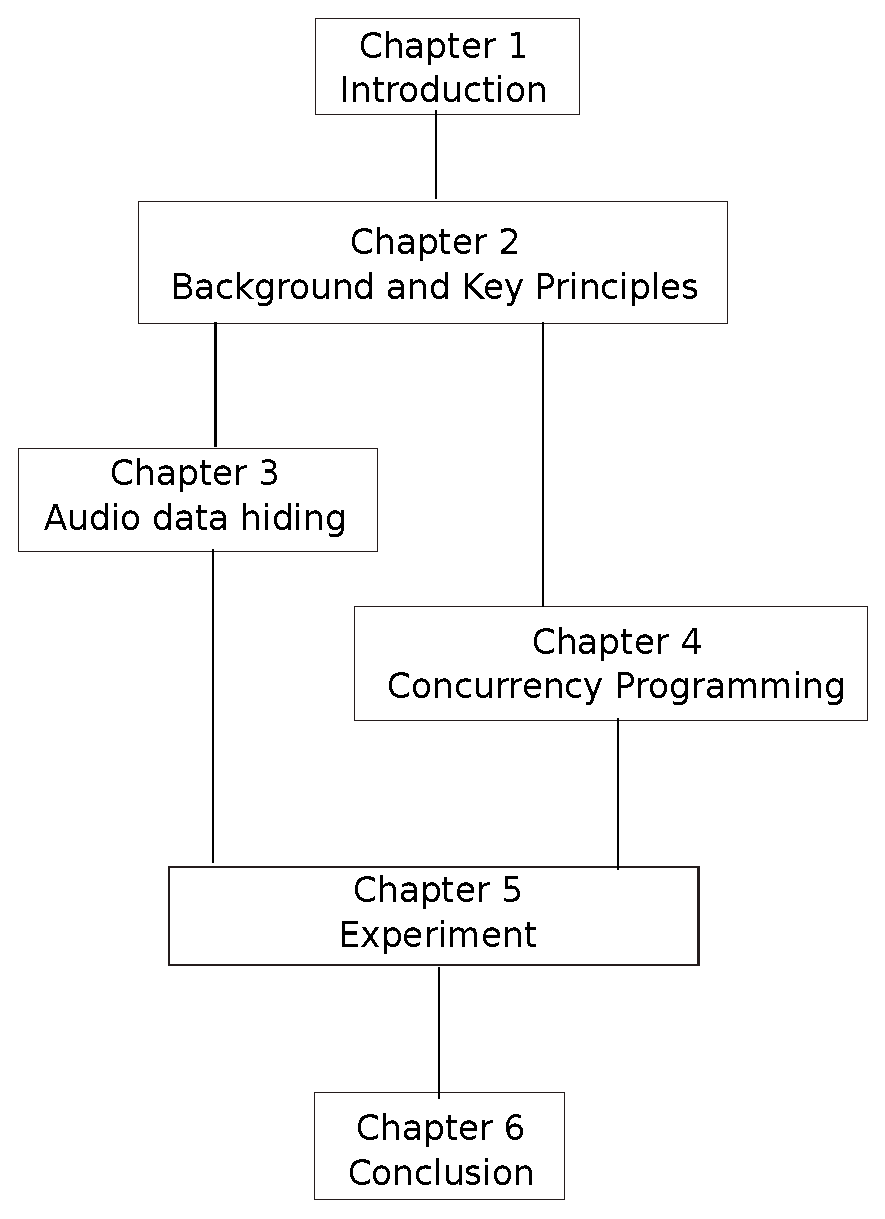
\includegraphics{drawing-2.eps}
  \caption{The schemantic overview of the thesis}
  \label{fig:ThesisOverview}
\end{figure}